\documentclass[9pt, pstricks, xcolor=dvipsnames]{beamer}

% ---------------- Configuración colores -----------------------
\usepackage{xcolor}
\definecolor{myprimary}{HTML}{a0c2b2}
\definecolor{mysecondary}{HTML}{809b8e}

\setbeamercolor{structure}{fg=myprimary}
\setbeamercolor{alerted text}{fg=mysecondary}

% ---------------- Configuración estilo -----------------------
\usetheme{Antibes}
\useoutertheme{miniframes}
\useinnertheme{circles}
\usecolortheme{beaver}
\usepackage{ragged2e}

\setbeamercolor{structure}{fg=myprimary}
\setbeamercolor{palette primary}{bg=myprimary,fg=white}
\setbeamercolor{palette secondary}{bg=myprimary,fg=white}
\setbeamercolor{palette tertiary}{bg=myprimary,fg=white}
\setbeamercolor{palette quaternary}{bg=myprimary,fg=white}
\setbeamercolor{structure}{fg=myprimary}
\setbeamercolor{section in toc}{fg=myprimary}
\setbeamercolor{subsection in head/foot}{bg=mysecondary,fg=white}
\setbeamercolor{title}{fg=white}
\setbeamercolor{subtitle}{fg=white}
\setbeamercolor{frametitle}{fg=mysecondary}

% ---------------- Configuración fuente -----------------------
\usefonttheme{structurebold}
\setbeamerfont{structure}{family=\sffamily} 
\usepackage{booktabs}

% ---------------- Configuración charts -----------------------
\usepackage{tikz}
\usepackage{calc}
\newlength{\outerradius}
\newlength{\innerradius}
\setlength{\outerradius}{2cm}
\setlength{\innerradius}{1.5cm}

\newcommand{\progresscircle}[1]{
  \begin{tikzpicture}
    \fill[myprimary] (0,0) circle (\outerradius);
    \fill[mysecondary] (0,0) -- (0, \outerradius)
      arc (90:90-3.6*#1:\outerradius) -- (0,0);
    \fill[white] (0,0) circle (\innerradius);
    \node (0,0) {\Huge\sffamily #1\%};
  \end{tikzpicture}
}

%\renewcommand{\labelenumi}{\SebastianoItem{\arabic{enumi}}}

% ---------------- Configuración listas -----------------------
\newcommand{\SebastianoItem}[1]{\tikz[baseline=(SebastianoItem.base),remember
picture]{%
\node[fill=myprimary!20,inner sep=4pt,font=\sffamily] (SebastianoItem){#1};}}
\newcommand{\SebastianoHighlight}{\tikz[overlay,remember picture]{%
\fill[myprimary!20] ([yshift=4pt,xshift=-\pgflinewidth]SebastianoItem.east) -- ++(4pt,-4pt)
-- ++(-4pt,-4pt) -- cycle;
}}

% -------------------- Configuración portada ---------------------
\title{\textbf{\textit{Android Malware Detection}}}
\subtitle{\textbf{Machine Learning I}}
\author{
    \small\href{mailto:abel.juncal@udc.es}{Abel Juncal Suárez} \\
    \small\href{mailto:alejandro.dopico2@udc.es}{Alejandro Dopico Castro} \\
    \small\href{mailto:javier.toron@udc.es}{Javier Torón Artiles} \\
    \small\href{mailto:lucia.maria.alvarez.crespo@udc.es}{Lucía María Álvarez Crespo}
    }

\institute{\textsc{\small Master in Artificial Intelligence 2023/2024}
    \and
    \textsc{\small Group C}}
\date{\footnotesize\today}

\begin{document}

\begin{frame}
	\titlepage
\end{frame}

%------------------------------------------------------

% \begin{frame}
% \frametitle{Table of contents}

% \tableofcontents
    
% \end{frame}

%------------------------------------------------------
\section{Introduction}
\frame{\insertsection}
\begin{frame}{Introduction}

\framesubtitle{The problem}

\begin{columns}
  \begin{column}{0.5\textwidth}
    \centering
    \progresscircle{70}
    \pause
  \end{column}
  \begin{column}{0.5\textwidth}
    \centering
    
\includegraphics[scale=0.2]{images/warning.png}
  \end{column}
\end{columns}

\end{frame}

%------------------------------------------------------

\begin{frame}{Introduction}
\framesubtitle{About the dataset}

\begin{enumerate}
    \pause
    \item 355,630 rows
    \pause
    \item 86 columns
    \pause
    \item 4 classes
        \pause
        \begin{itemize}
            \item Android Adware
            \pause
            \item Android Scareware
            \pause
            \item Android SMS Malware
            \pause
            \item Benign
        \end{itemize}
    \pause
    \item Network flow characteristics
    \pause
    \item Statistics of android apps behaviour
        \pause
        \begin{itemize}
            \item IP (source and dest)
            \pause
            \item Ports
            \pause
            \item Protocol
            \pause
            \item Packets details
        \end{itemize}
  \end{enumerate}

\pause

% \begin{columns}
% \column{0.6\textwidth}
%     \begin{itemize}
%         \item 355,630 rows
%         \item 86 columns
%         \item 4 classes
%         \begin{itemize}
%             \item Android Adware
%             \item Android Scareware
%             \item Android SMS Malware
%             \item Benign
%         \end{itemize}
%         \item Network flow characteristics
%         \item Statistics of android apps behaviour
%         \begin{itemize}
%             \item IP (source and dest)
%             \item Ports
%             \item Protocol
%             \item Packets details
%         \end{itemize}
%     \end{itemize}
    

% \column{0.65\textwidth}
%     \begin{figure}
%         \centering
%         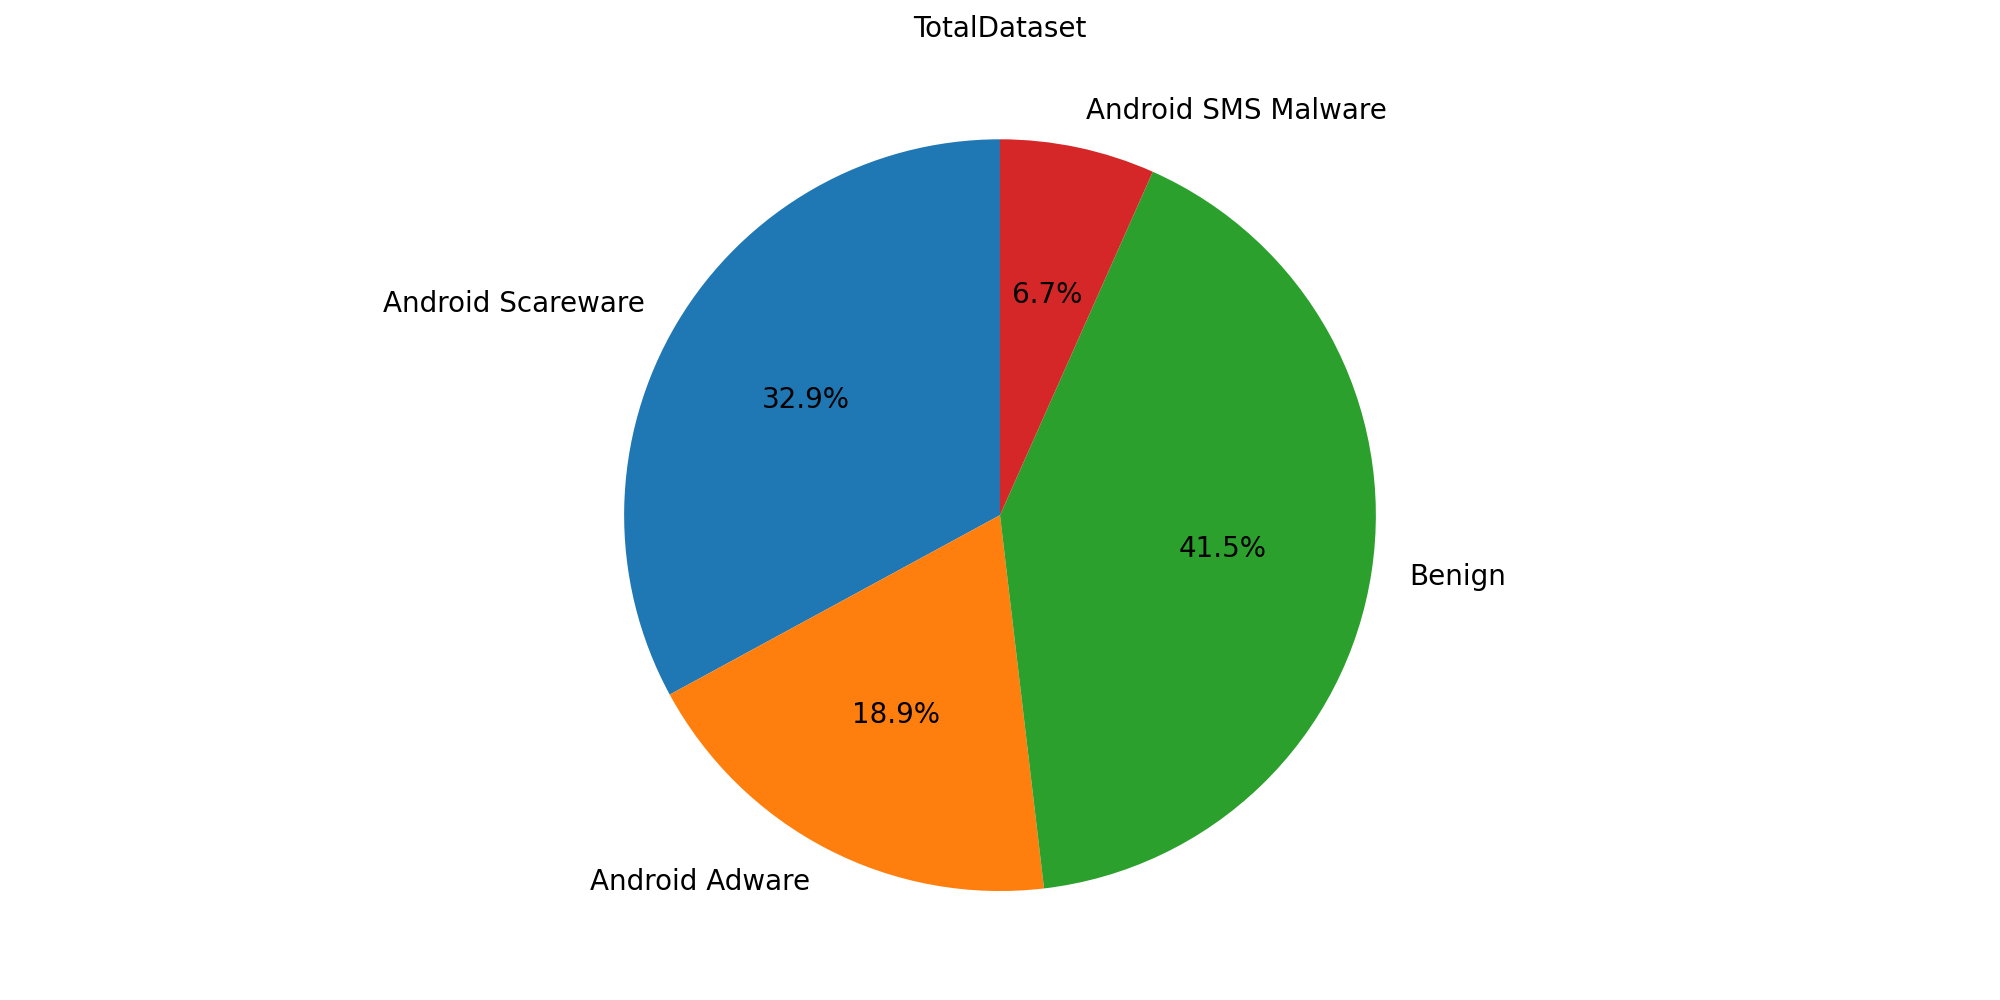
\includegraphics[width=\textwidth]{images/datasetPieChart.png} % Hay que cambiar esto, esta al reves.
%     \end{figure}
    
% \end{columns}
\end{frame}

%------------------------------------------------------
\begin{frame}{Introduction}
\framesubtitle{Dataset}

\begin{table}[h!]
\centering
\begin{tabular}{lll}
\hline
Label                 & Dataset Entries & Used Entries\\ \hline
Android\_Adware       & 147,443         & 1,475\\
Android\_Scareware    & 117,082         & 1,171\\
Android\_SMS\_Malware & 67,397          & 674\\
Benign                & 23,708          & 237\\ \hline
Total size            & 355,630                & 3,557\\ \hline
\end{tabular}
% \caption{Distribution of the dataset}
\label{tab:table}
\end{table}


\end{frame}
%------------------------------------------------------
\section{Approaches}
\frame{\insertsection}
\begin{frame}{Approach 1: Binary Classification}
\framesubtitle{Data Preprocessing}

\begin{columns}
  \begin{column}{0.5\textwidth}
    \centering
    \progresscircle{7}
    \pause
  \end{column}
  \begin{column}{0.5\textwidth}
    \centering
    \begin{tabular}{ll}
     \hline
     Label       & Entries \\ \hline
     Benign      & 237  \\ 
     Malware     & 3,320 \\ \hline
     Total size  & 3,557 \\ \hline
     \end{tabular}
  \end{column}
\end{columns}

\end{frame}

%------------------------------------------------------
\begin{frame}{Approach 1: Binary Classification}
\framesubtitle{Results: ANN CV}

\begin{table}[h]
    \centering
    \begin{tabular}{lcccc}
        \toprule
        Architecture & Accuracy & Recall & Specificity & F1-Score \\
        \midrule
        20 & 93.71\% \textit{(0.0)} & 100.0\% \textit{(0.0)} & 0.0\% \textit{(0.0)} & 96.75\% \textit{(0.0)} \\
        40 & 93.71\% \textit{(0.0)} & 100.0\% \textit{(0.0)} & 0.0\% \textit{(0.0)} & 96.75\% \textit{(0.0)} \\
        80 & 93.71\% \textit{(0.0)} & 100.0\% \textit{(0.0)} & 0.0\% \textit{(0.0)} & 96.75\% \textit{(0.0)} \\
        100 & 93.71\% \textit{(0.0)} & 100.0\% \textit{(0.0)} & 0.0\% \textit{(0.0)} & 96.75\% \textit{(0.0)} \\
        60, 120 & 93.71\% \textit{(0.0)} & 100.0\% \textit{(0.0)} & 0.0\% \textit{(0.0)} & 96.75\% \textit{(0.0)} \\
        80, 50 & 93.71\% \textit{(0.0)} & 100.0\% \textit{(0.0)} & 0.0\% \textit{(0.0)} & 96.75\% \textit{(0.0)} \\
        80, 100 & 93.71\% \textit{(0.0)} & 100.0\% \textit{(0.0)} & 0.0\% \textit{(0.0)} & 96.75\% \textit{(0.0)} \\
        100, 40 & 93.71\% \textit{(0.0)} & 100.0\% \textit{(0.0)} & 0.0\% \textit{(0.0)} & 96.75\% \textit{(0.0)} \\
        \bottomrule
    \end{tabular}
    \caption{ANN metrics result for CrossValidation}
    \label{tab:ann_CV_approach1}
    \end{table}

\end{frame}

%------------------------------------------------------
\begin{frame}{Approach 1: Binary Classification}
\framesubtitle{Results: ANN}
\begin{table}[H]
    \centering
    \begin{tabular}{lccccc}
        \toprule
        Architecture & Accuracy & Recall & Specificity & F1-Score & CM\\
        \midrule
        20 & 91.85\%  & 100.0\%  & 0.0\%  & 95.75\% & [654 58; 0 0] \\
        40 & 91.85\%  & 100.0\%  & 0.0\%  & 95.75\% & [654 58; 0 0] \\
        80 & 91.85\%  & 100.0\%  & 0.0\%  & 95.75\% & [654 58; 0 0] \\
        100 & 91.85\%  & 100.0\%  & 0.0\%  & 95.75\% & [654 58; 0 0] \\
        60, 120 & 91.85\%  & 100.0\%  & 0.0\%  & 95.75\% & [654 58; 0 0] \\
        80, 50 & 91.85\%  & 100.0\%  & 0.0\%  & 95.75\% & [654 58; 0 0] \\
        80, 100 & 91.85\%  & 100.0\%  & 0.0\%  & 95.75\% & [654 58; 0 0] \\
        100, 40 & 91.85\%  & 100.0\%  & 0.0\%  & 95.75\% & [654 58; 0 0] \\

        \bottomrule
    \end{tabular}
    \caption{ANN metrics result}
    \label{tab:ann_approach1}
\end{table}
\end{frame}
%------------------------------------------------------
\begin{frame}{Approach 1: Binary Classification}
\framesubtitle{Results: kNN CV}
\begin{table}[H]
    \centering
    \begin{tabular}{lcccc}
        \toprule
        k          & Accuracy                & Recall                   & Specificity               & F1-Score  \\
        \midrule
        1 & 88.08\% \textit{(0.01)} & 93.17\% \textit{(0.01)} & 12.29\% \textit{(0.08)} & 93.61\% \textit{(0.01)} \\
        2 & 83.3\% \textit{(0.01)} & 87.66\% \textit{(0.02)} & 18.43\% \textit{(0.11)} & 90.77\% \textit{(0.01)} \\
        3 & 92.72\% \textit{(0.01)} & 98.84\% \textit{(0.01)} & 1.7\% \textit{(0.03)} & 96.22\% \textit{(0.0)} \\
        5 & 93.5\% \textit{(0.0)} & 99.74\% \textit{(0.0)} & 0.56\% \textit{(0.02)} & 96.64\% \textit{(0.0)} \\
        7 & 93.6\% \textit{(0.0)} & 99.89\% \textit{(0.0)} & 0.0\% \textit{(0.0)} & 96.7\% \textit{(0.0)} \\
        10 & 93.6\% \textit{(0.0)} & 99.89\% \textit{(0.0)} & 0.0\% \textit{(0.0)} & 96.7\% \textit{(0.0)} \\
        15 & 93.71\% \textit{(0.0)} & 100.0\% \textit{(0.0)} & 0.0\% \textit{(0.0)} & 96.75\% \textit{(0.0)} \\

        \bottomrule
    \end{tabular}
    \caption{kNN metrics result for CrossValidation}
    \label{tab:kNN_CV_approach1}
\end{table}
\end{frame}
%------------------------------------------------------
\begin{frame}{Approach 1: Binary Classification}
\framesubtitle{Results: kNN}
\begin{table}[H]
    \centering
    \begin{tabular}{lccccc}
        \toprule
        k & Accuracy & Recall & Specificity & F1-Score & CM \\
        \midrule
        1 & 87.22\%  & 94.19\%  & 8.62\%  & 93.12\% & [616 53; 38 5] \\
        2 & 80.48\%  & 86.39\%  & 13.79\%  & 89.05\% & [565 50; 89 8] \\
        3 & 90.03\%  & 97.86\%  & 1.72\%  & 94.74\% & [640 57; 14 1] \\
        5 & 91.43\%  & 99.54\%  & 0.0\%  & 95.52\% & [651 58; 3 0] \\
        7 & 91.85\%  & 100.0\%  & 0.0\%  & 95.75\% & [654 58; 0 0] \\
        10 & 91.85\%  & 100.0\%  & 0.0\%  & 95.75\% & [654 58; 0 0] \\
        15 & 91.85\%  & 100.0\%  & 0.0\%  & 95.75\% & [654 58; 0 0] \\
        \bottomrule
    \end{tabular}
    \caption{kNN metrics result}
    \label{tab:kNN_approach1}
\end{table}
\end{frame}
%------------------------------------------------------
\begin{frame}{Approach 1: Binary Classification}
\framesubtitle{Results: Decision Tree CV}
\begin{table}[H]
    \centering
    \begin{tabular}{lcccc}
        \toprule
        MaxDepth & Accuracy & Recall & Specificity & F1-Score  \\
        \midrule
        3 & 93.6\% \textit{(0.0)} & 99.89\% \textit{(0.0)} & 0.0\% \textit{(0.0)} & 96.7\% \textit{(0.0)} \\
        5 & 93.15\% \textit{(0.0)} & 99.36\% \textit{(0.0)} & 0.56\% \textit{(0.02)} & 96.45\% \textit{(0.0)} \\
        7 & 92.34\% \textit{(0.0)} & 98.39\% \textit{(0.0)} & 2.22\% \textit{(0.03)} & 96.01\% \textit{(0.0)} \\
        10 & 91.42\% \textit{(0.01)} & 97.22\% \textit{(0.01)} & 5.03\% \textit{(0.04)} & 95.5\% \textit{(0.01)} \\
        15 & 88.96\% \textit{(0.01)} & 94.26\% \textit{(0.02)} & 10.03\% \textit{(0.06)} & 94.11\% \textit{(0.01)} \\
        nothing & 87.1\% \textit{(0.02)} & 92.08\% \textit{(0.02)} & 12.88\% \textit{(0.08)} & 93.04\% \textit{(0.01)} \\

        \bottomrule
    \end{tabular}
    \caption{Decision Tree metrics result for CrossValidation}
    \label{tab:DT_CV_approach1}
\end{table}
\end{frame}
%------------------------------------------------------
\begin{frame}{Approach 1: Binary Classification}
\framesubtitle{Results: Decision Tree}
\begin{table}[H]
    \centering
    \begin{tabular}{lccccc}
        \toprule
        MaxDepth & Accuracy & Recall & Specificity & F1-Score & CM \\
        \midrule
        3 & 91.85\%  & 100.0\%  & 0.0\%  & 95.75\% & [654 58; 0 0] \\
        5 & 91.71\%  & 99.85\%  & 0.0\%  & 95.68\% & [653 58; 1 0] \\
        7 & 89.61\%  & 97.55\%  & 0.0\%  & 94.52\% & [638 58; 16 0] \\
        10 & 88.06\%  & 95.72\%  & 1.72\%  & 93.64\% & [626 57; 28 1] \\
        15 & 85.25\%  & 92.66\%  & 1.72\%  & 92.03\% & [606 57; 48 1] \\
        nothing & 84.55\%  & 91.9\%  & 1.72\%  & 91.62\% & [601 57; 53 1] \\
        \bottomrule
    \end{tabular}
    \caption{Decision Tree metrics result}
    \label{tab:dt_approach1}
\end{table}
\end{frame}
%------------------------------------------------------
\begin{frame}{Approach 1: Binary Classification}
\framesubtitle{Results: SVM CV}
\begin{table}[H]
    \centering
    \begin{tabular}{llcccc}
        \toprule
        Kernel & C & Accuracy & Recall & Specificity & F1-Score  \\
        \midrule
        rbf & 0.1 & 93.71\% \textit{(0.0)} & 100.0\% \textit{(0.0)} & 0.0\% \textit{(0.0)} & 96.75\% \textit{(0.0)} \\
        rbf & 1.0 & 93.71\% \textit{(0.0)} & 100.0\% \textit{(0.0)} & 0.0\% \textit{(0.0)} & 96.75\% \textit{(0.0)} \\
        rbf & 10.0 & 93.6\% \textit{(0.0)} & 99.89\% \textit{(0.0)} & 0.0\% \textit{(0.0)} & 96.7\% \textit{(0.0)} \\
        poly & 0.1 & 93.71\% \textit{(0.0)} & 100.0\% \textit{(0.0)} & 0.0\% \textit{(0.0)} & 96.75\% \textit{(0.0)} \\
        poly & 1.0 & 93.67\% \textit{(0.0)} & 99.96\% \textit{(0.0)} & 0.0\% \textit{(0.0)} & 96.73\% \textit{(0.0)} \\
        linear & 0.1 & 93.71\% \textit{(0.0)} & 100.0\% \textit{(0.0)} & 0.0\% \textit{(0.0)} & 96.75\% \textit{(0.0)} \\
        linear & 1.0 & 93.71\% \textit{(0.0)} & 100.0\% \textit{(0.0)} & 0.0\% \textit{(0.0)} & 96.75\% \textit{(0.0)} \\
        linear & 10.0 & 93.71\% \textit{(0.0)} & 100.0\% \textit{(0.0)} & 0.0\% \textit{(0.0)} & 96.75\% \textit{(0.0)} \\
        \bottomrule
    \end{tabular}
    \caption{SVM metrics result for CrossValidation}
    \label{tab:SVM_CV_approach1}
\end{table}
\end{frame}
%------------------------------------------------------
\begin{frame}{Approach 1: Binary Classification}
\framesubtitle{Results: SVM}
\begin{table}[H]
    \centering
    \begin{tabular}{llccccc}
        \toprule
        Kernel & C & Accuracy & Recall & Specificity & F1-Score & CM \\
        \midrule
        rbf & 0.1 & 91.85\%  & 100.0\%  & 0.0\%  & 95.75\% & [654 58; 0 0] \\
        rbf & 1.0 & 91.85\%  & 100.0\%  & 0.0\%  & 95.75\% & [654 58; 0 0] \\
        rbf & 10.0 & 91.71\%  & 99.85\%  & 0.0\%  & 95.68\% & [653 58; 1 0] \\
        poly & 0.1 & 91.85\%  & 100.0\%  & 0.0\%  & 95.75\% & [654 58; 0 0] \\
        poly & 1.0 & 91.71\%  & 99.85\%  & 0.0\%  & 95.68\% & [653 58; 1 0] \\
        linear & 0.1 & 91.85\%  & 100.0\%  & 0.0\%  & 95.75\% & [654 58; 0 0] \\
        linear & 1.0 & 91.85\%  & 100.0\%  & 0.0\%  & 95.75\% & [654 58; 0 0] \\
        linear & 10.0 & 91.85\%  & 100.0\%  & 0.0\%  & 95.75\% & [654 58; 0 0] \\
        \bottomrule
    \end{tabular}
    \caption{SVM metrics result}
    \label{tab:SVM_approach1}

\end{table}
\end{frame}
%------------------------------------------------------
\begin{frame}{Approach 1: Binary Classification}
\framesubtitle{Results: Ensemble Model CV}
\begin{table}[H]
    \centering
    \resizebox{\columnwidth}{!}{%
    \begin{tabular}{llcccc}
        \toprule
        Ensemble Model & Parameters & Accuracy & Recall & Specificity & F1-Score  \\
        \midrule
        Voting Hard & & 92.93\% \textit{(0.0)} & 99.06\% \textit{(0.01)} & 1.7\% \textit{(0.03)} & 96.33\% \textit{(0.0)} \\
        Stacking (DecisionTree) & Max Depth 10 & 92.06\% \textit{(0.01)} & 98.16\% \textit{(0.02)} & 1.11\% \textit{(0.02)} & 95.86\% \textit{(0.01)} \\
        Stacking (kNN) & numNeighboors = 2 & 82.88\% \textit{(0.04)} & 87.96\% \textit{(0.04)} & 7.32\% \textit{(0.09)} & 90.54\% \textit{(0.03)} \\
        Stacking (SVM) & C = 0.1, kernel = rbf & 93.71\% \textit{(0.0)} & 100.0\% \textit{(0.0)} & 0.0\% \textit{(0.0)} & 96.75\% \textit{(0.0)} \\
        \bottomrule
    \end{tabular}%
    }
    \caption{Ensemble Model metrics result for CrossValidation}
    \label{tab:EM_CV_approach1}
\end{table}
\end{frame}
%------------------------------------------------------
\begin{frame}{Approach 1: Binary Classification}
\framesubtitle{Results: Ensemble Model}
\begin{table}[H]
    \centering
    \resizebox{\columnwidth}{!}{%

    \begin{tabular}{llcccccc}
        \toprule
        Ensemble Model & Final Estimator & Accuracy & Recall & Specificity & F1-Score & CM  \\
        \midrule
        Voting Hard &  & 91.15\%  & 99.08\%  & 1.72\%  & 95.36\% & [648 57; 6 1] \\
        Stacking (DecisionTree) & Max Depth 10  & 90.59\%  & 98.62\%  & 0.0\%  & 95.06\% & [645 58; 9 0] \\
        Stacking (kNN) & numNeighboors = 2 & 81.18\%  & 87.16\%  & 13.79\%  & 89.48\% & [570 50; 84 8] \\
        Stacking (SVM) & C = 0.1, kernel = rbf & 91.85\%  & 100.0\%  & 0.0\%  & 95.75\% & [654 58; 0 0] \\
        \bottomrule
    \end{tabular}%
    }
    \caption{Ensemble Model metrics result}
    \label{tab:EM_approach1}
\end{table}
\end{frame}
%------------------------------------------------------
\begin{frame}{Approach 2: Binary Classification
with Balanced Classes}
\framesubtitle{Data Preprocessing}
\pause
\begin{columns}
    \begin{column}{0.5\textwidth}
        \begin{figure}
            \centering
            
\includegraphics[width=0.8\textwidth]{images/load-balancer.png}
            %\caption{Balanced classes}
        \end{figure}
    \end{column}
    \begin{column}{0.5\textwidth}
        \pause
        \centering
        \begin{table}[h!]
            \centering
            \begin{tabular}{ll}
                \hline
                Label                 & Entries \\ \hline
                Benign                &   3,320  \\ 
                Malware               &   3,320  \\ \hline
                Total size            &   6,640  \\ \hline
            \end{tabular}
        \end{table}
    \end{column}
\end{columns}



\end{frame}
%------------------------------------------------------
\begin{frame}{Approach 2: Binary Classification
with Balanced Classes}
\framesubtitle{Results: ANN CV}
\begin{table}[h]
    \centering
    \begin{tabular}{lcccc}
        \toprule
        Architecture & Accuracy & Recall & Specificity & F1-Score \\
        \midrule
        20 & 60.88\% \textit{(0.02)} & 58.13\% \textit{(0.02)} & 63.63\% \textit{(0.04)} & 59.48\% \textit{(0.01)} \\
        40 & 59.06\% \textit{(0.01)} & 56.72\% \textit{(0.03)} & 61.41\% \textit{(0.05)} & 56.85\% \textit{(0.02)} \\
        80 & 55.24\% \textit{(0.01)} & 56.49\% \textit{(0.04)} & 53.99\% \textit{(0.04)} & 52.61\% \textit{(0.02)} \\
        100 & 54.47\% \textit{(0.01)} & 52.87\% \textit{(0.04)} & 56.06\% \textit{(0.05)} & 49.85\% \textit{(0.02)} \\
        60, 120 & 53.94\% \textit{(0.01)} & 59.53\% \textit{(0.08)} & 48.36\% \textit{(0.09)} & 49.12\% \textit{(0.04)} \\
        80, 50 & 56.5\% \textit{(0.01)} & 56.82\% \textit{(0.04)} & 56.19\% \textit{(0.04)} & 52.23\% \textit{(0.01)} \\
        80, 100 & 54.67\% \textit{(0.01)} & 55.69\% \textit{(0.05)} & 53.65\% \textit{(0.06)} & 47.75\% \textit{(0.03)} \\
        100, 40 & 56.83\% \textit{(0.01)} & 59.17\% \textit{(0.06)} & 54.49\% \textit{(0.08)} & 53.57\% \textit{(0.03)} \\
        \bottomrule
    \end{tabular}
    \caption{ANN metrics result for CrossValidation}
    \label{tab:ann_CV_approach2}
\end{table}
\end{frame}
%------------------------------------------------------

\begin{frame}{Approach 2: Binary Classification
with Balanced Classes}
\framesubtitle{Results: ANN}
\begin{table}[H]
    \centering
    \begin{tabular}{lccccc}
        \toprule
        Architecture & Accuracy & Recall & Specificity & F1-Score & CM\\
        \midrule
        20 & 59.64\%  & 64.31\%  & 54.97\%  & 61.44\% & [427 299; 237 365] \\
        40 & 57.23\%  & 77.41\%  & 37.05\%  & 64.41\% & [514 418; 150 246] \\
        80 & 54.29\%  & 72.74\%  & 35.84\%  & 61.41\% & [483 426; 181 238] \\
        100 & 52.79\%  & 62.5\%  & 43.07\%  & 56.97\% & [415 378; 249 286] \\
        60, 120 & 54.44\%  & 16.27\%  & 92.62\%  & 26.31\% & [108 49; 556 615] \\
        80, 50 & 53.77\%  & 11.14\%  & 96.39\%  & 19.42\% & [74 24; 590 640] \\
        80, 100 & 56.55\%  & 25.0\%  & 88.1\%  & 36.52\% & [166 79; 498 585] \\
        100, 40 & 58.89\%  & 83.89\%  & 33.89\%  & 67.11\% & [557 439; 107 225] \\
        \bottomrule
    \end{tabular}
    \caption{ANN metrics result}
    \label{tab:ann_approach2}
\end{table}
\end{frame}
%------------------------------------------------------
\begin{frame}{Approach 2: Binary Classification
with Balanced Classes}
\framesubtitle{Results: kNN CV}
\begin{table}[H]
    \centering
    \begin{tabular}{lcccc}
        \toprule
        k          & Accuracy                & Recall                   & Specificity               & F1-Score  \\
        \midrule
        1 & 95.33\% \textit{(0.01)} & 90.66\% \textit{(0.02)} & 100.0\% \textit{(0.0)} & 95.1\% \textit{(0.01)} \\
        2 & 91.3\% \textit{(0.01)} & 82.6\% \textit{(0.02)} & 100.0\% \textit{(0.0)} & 90.46\% \textit{(0.01)} \\
        3 & 91.3\% \textit{(0.01)} & 82.6\% \textit{(0.02)} & 100.0\% \textit{(0.0)} & 90.46\% \textit{(0.01)} \\
        5 & 87.71\% \textit{(0.01)} & 75.41\% \textit{(0.02)} & 100.0\% \textit{(0.0)} & 85.97\% \textit{(0.01)} \\
        7 & 83.98\% \textit{(0.01)} & 67.96\% \textit{(0.03)} & 100.0\% \textit{(0.0)} & 80.89\% \textit{(0.02)} \\
        10 & 77.97\% \textit{(0.01)} & 56.06\% \textit{(0.03)} & 99.89\% \textit{(0.0)} & 71.76\% \textit{(0.02)} \\
        15 & 72.36\% \textit{(0.01)} & 48.87\% \textit{(0.02)} & 95.86\% \textit{(0.02)} & 63.86\% \textit{(0.02)} \\
        \bottomrule
    \end{tabular}
    \caption{kNN metrics result for CrossValidation}
    \label{tab:kNN_CV_approach2}
\end{table}
\end{frame}
%------------------------------------------------------
\begin{frame}{Approach 2: Binary Classification
with Balanced Classes}
\framesubtitle{Results: kNN}
\begin{table}[H]
    \centering
    \begin{tabular}{lccccc}
        \toprule
        k & Accuracy & Recall & Specificity & F1-Score & CM \\
        \midrule
        1 & 96.01\%  & 92.02\%  & 100.0\%  & 95.84\% & [611 0; 53 664] \\
        2 & 91.49\%  & 82.98\%  & 100.0\%  & 90.7\% & [551 0; 113 664] \\
        3 & 91.49\%  & 82.98\%  & 100.0\%  & 90.7\% & [551 0; 113 664] \\
        5 & 87.73\%  & 75.45\%  & 100.0\%  & 86.01\% & [501 0; 163 664] \\
        7 & 85.02\%  & 70.03\%  & 100.0\%  & 82.37\% & [465 0; 199 664] \\
        10 & 80.12\%  & 60.24\%  & 100.0\%  & 75.19\% & [400 0; 264 664] \\
        15 & 74.7\%  & 50.45\%  & 98.95\%  & 66.6\% & [335 7; 329 657] \\
        \bottomrule
    \end{tabular}
    \caption{kNN metrics result}
    \label{tab:kNN_approach2}
\end{table}
\end{frame}
%------------------------------------------------------
\begin{frame}{Approach 2: Binary Classification
with Balanced Classes}
\framesubtitle{Results: Decision Tree CV}
\begin{table}[H]
\centering
\begin{tabular}{lcccc}
\toprule
MaxDepth & Accuracy & Recall & Specificity & F1-Score \\
\midrule
3 & 56.85\% \textit{(0.02)} & 42.33\% \textit{(0.22)} & 71.37\% \textit{(0.22)} & 46.65\% \textit{(0.13)} \\
5 & 61.8\% \textit{(0.02)} & 42.16\% \textit{(0.12)} & 81.44\% \textit{(0.14)} & 51.67\% \textit{(0.06)} \\
7 & 67.28\% \textit{(0.02)} & 51.42\% \textit{(0.13)} & 83.14\% \textit{(0.09)} & 60.14\% \textit{(0.08)} \\
10 & 77.59\% \textit{(0.03)} & 64.57\% \textit{(0.08)} & 90.62\% \textit{(0.05)} & 74.01\% \textit{(0.05)} \\
15 & 88.57\% \textit{(0.02)} & 78.77\% \textit{(0.04)} & 98.38\% \textit{(0.01)} & 87.28\% \textit{(0.03)} \\
None & 95.29\% \textit{(0.01)} & 90.59\% \textit{(0.02)} & 100.0\% \textit{(0.0)} & 95.05\% \textit{(0.01)} \\
\bottomrule
\end{tabular}
\caption{Decision Tree metrics result for CrossValidation}
\label{tab:DT_CV_approach2}
\end{table}
\end{frame}
%------------------------------------------------------
\begin{frame}{Approach 2: Binary Classification
with Balanced Classes}
\framesubtitle{Results: Decision Tree}
\begin{table}[H]
\centering
\begin{tabular}{lccccc}
\toprule
MaxDepth & Accuracy & Recall & Specificity & F1-Score & CM \\
\midrule
3 & 58.89\%  & 43.52\%  & 74.25\%  & 51.42\% & [289 171; 375 493] \\
5 & 63.03\%  & 49.55\%  & 76.51\%  & 57.27\% & [329 156; 335 508] \\
7 & 71.23\%  & 58.73\%  & 83.73\%  & 67.13\% & [390 108; 274 556] \\
10 & 81.4\%  & 65.81\%  & 96.99\%  & 77.97\% & [437 20; 227 644] \\
15 & 91.04\%  & 82.08\%  & 100.0\%  & 90.16\% & [545 0; 119 664] \\
None & 96.31\%  & 92.62\%  & 100.0\%  & 96.17\% & [615 0; 49 664] \\
\bottomrule
\end{tabular}
\caption{Decision Tree metrics result}
\label{tab:dt_approach2}
\end{table}
\end{frame}
%------------------------------------------------------
\begin{frame}{Approach 2: Binary Classification
with Balanced Classes}
\framesubtitle{Results: SVM CV}
\begin{table}[H]
\centering
\begin{tabular}{llcccc}
\toprule
Kernel & C & Accuracy & Recall & Specificity & F1-Score \\
\midrule
rbf & 0.1 & 57.27\% \textit{(0.03)} & 62.57\% \textit{(0.03)} & 51.96\% \textit{(0.06)} & 59.43\% \textit{(0.02)} \\
rbf & 1.0 & 64.19\% \textit{(0.03)} & 58.09\% \textit{(0.04)} & 70.3\% \textit{(0.05)} & 61.83\% \textit{(0.03)} \\
rbf & 10.0 & 71.74\% \textit{(0.02)} & 64.34\% \textit{(0.04)} & 79.14\% \textit{(0.04)} & 69.46\% \textit{(0.03)} \\
poly & 0.1 & 57.46\% \textit{(0.02)} & 90.14\% \textit{(0.02)} & 24.78\% \textit{(0.05)} & 67.95\% \textit{(0.01)} \\
poly & 1.0 & 62.07\% \textit{(0.03)} & 77.63\% \textit{(0.03)} & 46.5\% \textit{(0.06)} & 67.19\% \textit{(0.02)} \\
linear & 0.1 & 57.32\% \textit{(0.01)} & 56.81\% \textit{(0.05)} & 57.83\% \textit{(0.06)} & 57.0\% \textit{(0.02)} \\
linear & 1.0 & 58.74\% \textit{(0.01)} & 60.13\% \textit{(0.05)} & 57.35\% \textit{(0.06)} & 59.23\% \textit{(0.02)} \\
linear & 10.0 & 59.32\% \textit{(0.02)} & 62.72\% \textit{(0.04)} & 55.92\% \textit{(0.06)} & 60.63\% \textit{(0.02)} \\
\bottomrule
\end{tabular}
\caption{SVM metrics result for CrossValidation}
\label{tab:SVM_CV_approach2}
\end{table}
\end{frame}
%------------------------------------------------------
\begin{frame}{Approach 2: Binary Classification
with Balanced Classes}
\framesubtitle{Results: SVM}
\begin{table}[H]
\centering
\begin{tabular}{llccccc}
\toprule
Kernel & C & Accuracy & Recall & Specificity & F1-Score & CM \\
\midrule
rbf & 0.1 & 57.3\%  & 59.49\%  & 55.12\%  & 58.22\% & [395 298; 269 366] \\
rbf & 1.0 & 63.18\%  & 56.63\%  & 69.73\%  & 60.6\% & [376 201; 288 463] \\
rbf & 10.0 & 72.44\%  & 61.75\%  & 83.13\%  & 69.14\% & [410 112; 254 552] \\
poly & 0.1 & 56.78\%  & 89.31\%  & 24.25\%  & 67.39\% & [593 503; 71 161] \\
poly & 1.0 & 63.93\%  & 76.96\%  & 50.9\%  & 68.09\% & [511 326; 153 338] \\
linear & 0.1 & 58.51\%  & 54.52\%  & 62.5\%  & 56.78\% & [362 249; 302 415] \\
linear & 1.0 & 58.66\%  & 57.08\%  & 60.24\%  & 58.0\% & [379 264; 285 400] \\
linear & 10.0 & 59.19\%  & 60.54\%  & 57.83\%  & 59.73\% & [402 280; 262 384] \\
\bottomrule
\end{tabular}
\caption{SVM metrics result}
\label{tab:SVM_approach2}
\end{table}
\end{frame}
%------------------------------------------------------
\begin{frame}{Approach 2: Binary Classification
with Balanced Classes}
\framesubtitle{Results: Ensembles CV}
\begin{table}[H]
    \centering
    \resizebox{\columnwidth}{!}{%
    \begin{tabular}{llcccc}
        \toprule
        Ensemble Model & Parameters & Accuracy & Recall & Specificity & F1-Score  \\
        \midrule
        Hard Voting & &  94.33\% \textit{(0.01)} & 88.67\% \textit{(0.02)} & 100.0\% \textit{(0.0)} & 93.98\% \textit{(0.01)} \\
        Stacking (Decision Tree) & Max Depth = None & 97.27\% \textit{(0.01)} & 98.42\% \textit{(0.01)} & 96.12\% \textit{(0.02)} & 97.31\% \textit{(0.01)} \\
        Stacking (kNN) & numNeighboors = 1 & 97.27\% \textit{(0.01)} & 98.42\% \textit{(0.01)} & 96.12\% \textit{(0.02)} & 97.31\% \textit{(0.01)} \\
        Stacking (SVM) & C = 10, kernel = rbf & 99.1\% \textit{(0.0)} & 98.19\% \textit{(0.01)} & 100.0\% \textit{(0.0)} & 99.09\% \textit{(0.0)} \\
        \bottomrule
    \end{tabular}%
    }
    \caption{Ensemble Model metrics result for CrossValidation}
    \label{tab:EM_CV_approach2}
\end{table}
\end{frame}
%------------------------------------------------------
\begin{frame}{Approach 2: Binary Classification
with Balanced Classes}
\framesubtitle{Results: Ensembles}
\begin{table}[H]
    \centering
    \resizebox{\columnwidth}{!}{%
    \begin{tabular}{llcccccc}
        \toprule
        Ensemble Model & Final Estimator & Accuracy & Recall & Specificity & F1-Score & CM  \\
        \midrule
        Hard Voting & & 95.11\%  & 90.21\%  & 100.0\%  & 94.85\% & [599 0; 65 664] \\
        Stacking (Decision Tree) & Max Depth = None & 95.26\%  & 98.34\%  & 92.17\%  & 95.4\% & [653 52; 11 612] \\
        Stacking (kNN) & numNeighboors = 1 & 95.26\%  & 98.34\%  & 92.17\%  & 95.4\% & [653 52; 11 612] \\
        Stacking (SVM) & C = 10, kernel = rbf  & 99.02\%  & 98.04\%  & 100.0\%  & 99.01\% & [651 0; 13 664] \\
        \bottomrule
    \end{tabular}%
    }
    \caption{Ensemble Model metrics result}
    \label{tab:EM_approach2}
\end{table}
\end{frame}
%------------------------------------------------------
\begin{frame}{Approach 3: Multiclass Classification}
\framesubtitle{Data Preprocessing}
\pause
\begin{columns}
    \begin{column}{0.5\textwidth}
        \begin{figure}
            \centering
            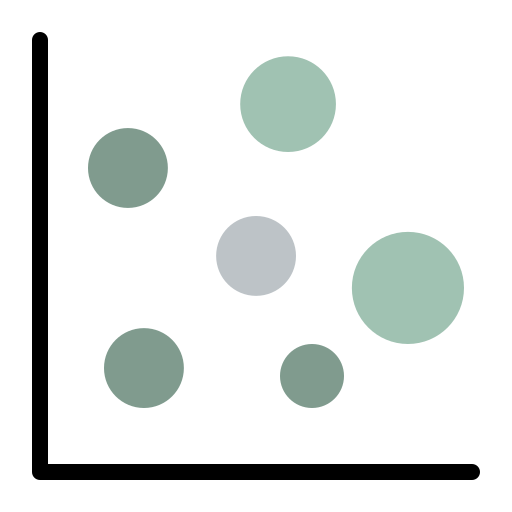
\includegraphics[width=0.8\textwidth]{images/chart-bullet.png}
            %\caption{Multiclass}
        \end{figure}
    \end{column}
    \begin{column}{0.5\textwidth}
        \pause
        \centering
        \begin{table}[h!]
            \centering
            \begin{tabular}{ll}
                \hline
        Label                 & Entries  \\ \hline
        Benign                &   1,475  \\ 
        Android\_Scareware    &   1,475  \\
        Android\_SMS\_Malware &   1,475  \\
        Android\_Adware       &   1,475  \\
        \hline
        Total size            &   5,900 \\ \hline
            \end{tabular}
        \end{table}
    \end{column}
\end{columns}

% \begin{table}[h!]
%     \centering
%     \begin{tabular}{ll}
%         \hline
%         Label                 & Entries  \\ \hline
%         Benign                &   1,475  \\ 
%         Android\_Scareware    &   1,475  \\
%         Android\_SMS\_Malware &   1,475  \\
%         Android\_Adware       &   1,475  \\
%         \hline
%         Total size            &   5,900 \\ \hline
%     \end{tabular}
%     \caption{Label distribution of the dataset in third approach}
%     \label{tab:dataset_distribution_third_approach}
% \end{table}

\end{frame}
%------------------------------------------------------
\begin{frame}{Approach 3: Multiclass Classification}
\framesubtitle{Results: ANN CV}
\begin{table}[H]
\centering
\begin{tabular}{lcccc}
\toprule
Architecture & Accuracy & Recall & Specificity & F1-Score \\\midrule
20 & 33.21\% \textit{(0.01)} & 33.21\% \textit{(0.01)} & 77.75\% \textit{(0.0)} & 32.2\% \textit{(0.01)} \\
40 & 32.82\% \textit{(0.01)} & 32.82\% \textit{(0.01)} & 77.61\% \textit{(0.0)} & 30.85\% \textit{(0.01)} \\
80 & 31.43\% \textit{(0.01)} & 31.43\% \textit{(0.01)} & 77.13\% \textit{(0.0)} & 27.34\% \textit{(0.01)} \\
100 & 30.83\% \textit{(0.01)} & 30.83\% \textit{(0.01)} & 76.95\% \textit{(0.0)} & 26.02\% \textit{(0.01)} \\
60, 120 & 30.2\% \textit{(0.0)} & 30.2\% \textit{(0.0)} & 76.71\% \textit{(0.0)} & 21.09\% \textit{(0.01)} \\
80, 50 & 31.67\% \textit{(0.01)} & 31.67\% \textit{(0.01)} & 77.22\% \textit{(0.0)} & 25.56\% \textit{(0.01)} \\
80, 100 & 30.12\% \textit{(0.01)} & 30.12\% \textit{(0.01)} & 76.71\% \textit{(0.0)} & 21.38\% \textit{(0.01)} \\
100, 40 & 31.61\% \textit{(0.01)} & 31.61\% \textit{(0.01)} & 77.21\% \textit{(0.0)} & 25.89\% \textit{(0.01)} \\


\bottomrule
\end{tabular}
\caption{ANN metrics result for CrossValidation}
\label{tab:ann_CV_approach3}
\end{table}

\end{frame}
%------------------------------------------------------
\begin{frame}{Approach 3: Multiclass Classification}
\framesubtitle{Results: ANN}
\begin{table}[H]
\centering
\resizebox{\textwidth}{!}{% Ajusta la tabla al ancho del texto
\begin{tabular}{lccccc}
\toprule
Architecture & Accuracy & Recall & Specificity & F1-Score & CM\\
\midrule
20 & 22.37\%  & 22.37\%  & 73.78\%  & 20.66\% & [67 104 105 26; 78 56 135 35; 76 64 124 32; 117 48 96 17] \\
40 & 20.59\%  & 20.59\%  & 72.99\%  & 17.85\% & [147 80 55 20; 166 35 68 35; 171 61 43 21; 175 48 37 18] \\
80 & 23.9\%  & 23.9\%  & 74.66\%  & 23.48\% & [78 87 51 86; 86 86 36 96; 69 97 41 89; 87 88 26 77] \\
100 & 21.44\%  & 21.44\%  & 73.11\%  & 17.1\% & [74 200 15 13; 105 155 12 32; 107 153 9 27; 128 120 15 15] \\
60, 120 & 23.64\%  & 23.64\%  & 75.28\%  & 17.65\% & [3 44 132 123; 7 12 137 148; 8 21 115 152; 8 18 103 149] \\
80, 50 & 21.44\%  & 21.44\%  & 74.18\%  & 16.98\% & [12 169 20 101; 28 99 10 167; 22 115 10 149; 31 101 14 132] \\
80, 100 & 25.42\%  & 25.42\%  & 74.6\%  & 17.27\% & [239 24 31 8; 208 7 65 24; 220 12 45 19; 219 7 43 9] \\
100, 40 & 23.9\%  & 23.9\%  & 75.43\%  & 17.48\% & [6 29 126 141; 12 5 139 148; 9 15 119 153; 20 8 98 152] \\
\bottomrule
\end{tabular}
}
\caption{ANN metrics result}
\label{tab:ann_approach3}
\end{table}
\end{frame}
%------------------------------------------------------
\begin{frame}{Approach 3: Multiclass Classification}
\framesubtitle{Results: kNN CV}
\begin{table}[H]
\centering
\begin{tabular}{lcccc}
\toprule
k & Accuracy & Recall & Specificity & F1-Score \\
\midrule
1 & 71.65\% \textit{(0.02)} & 71.65\% \textit{(0.02)} & 90.54\% \textit{(0.01)} & 70.28\% \textit{(0.02)} \\
2 & 62.31\% \textit{(0.02)} & 62.31\% \textit{(0.02)} & 87.44\% \textit{(0.01)} & 60.55\% \textit{(0.02)} \\
3 & 57.35\% \textit{(0.02)} & 57.35\% \textit{(0.02)} & 85.78\% \textit{(0.01)} & 55.48\% \textit{(0.02)} \\
5 & 52.04\% \textit{(0.02)} & 52.04\% \textit{(0.02)} & 84.0\% \textit{(0.01)} & 49.75\% \textit{(0.02)} \\
7 & 47.67\% \textit{(0.03)} & 47.67\% \textit{(0.03)} & 82.57\% \textit{(0.01)} & 45.61\% \textit{(0.03)} \\
10 & 41.42\% \textit{(0.03)} & 41.42\% \textit{(0.03)} & 80.48\% \textit{(0.01)} & 40.28\% \textit{(0.03)} \\
15 & 39.47\% \textit{(0.03)} & 39.47\% \textit{(0.03)} & 79.83\% \textit{(0.01)} & 38.99\% \textit{(0.03)} \\
\bottomrule
\end{tabular}
\caption{kNN metrics result for CrossValidation}
\label{tab:kNN_CV_approach3}
\end{table}
\end{frame}
%------------------------------------------------------
\begin{frame}{Approach 3: Multiclass Classification}
\framesubtitle{Results: kNN}
\begin{table}[H]
\centering
\resizebox{\textwidth}{!}{% Ajusta la tabla al ancho del texto
\begin{tabular}{lccccc}
\toprule
k & Accuracy & Recall & Specificity & F1-Score & CM \\
\midrule
1 & 71.78\%  & 71.78\%  & 90.64\%  & 70.38\% & [302 0 0 0; 22 143 85 54; 14 86 154 42; 4 10 16 248] \\
2 & 63.73\%  & 63.73\%  & 87.91\%  & 61.89\% & [297 5 0 0; 22 172 45 65; 14 133 82 67; 4 67 6 201] \\
3 & 57.97\%  & 57.97\%  & 86.01\%  & 56.11\% & [297 5 0 0; 35 127 70 72; 43 85 100 68; 17 62 39 160] \\
5 & 56.19\%  & 56.19\%  & 85.36\%  & 54.22\% & [285 5 8 4; 46 128 68 62; 65 72 100 59; 35 53 40 150] \\
7 & 50.42\%  & 50.42\%  & 83.37\%  & 48.24\% & [270 14 8 10; 67 112 73 52; 81 72 87 56; 48 54 50 126] \\
10 & 43.98\%  & 43.98\%  & 81.21\%  & 42.53\% & [216 30 28 28; 84 109 60 51; 91 72 74 59; 52 58 48 120] \\
15 & 40.0\%  & 40.0\%  & 79.94\%  & 39.13\% & [182 36 46 38; 78 100 72 54; 81 70 75 70; 66 49 48 115] \\
\bottomrule
\end{tabular}
}
\caption{kNN metrics result}
\label{tab:kNN_approach3}
\end{table}
\end{frame}
%------------------------------------------------------
\begin{frame}{Approach 3: Multiclass Classification}
\framesubtitle{Results: Decision Tree CV}
\begin{table}[H]
\centering
\begin{tabular}{lcccc}
\toprule
MaxDepth & Accuracy & Recall & Specificity & F1-Score \\
\midrule
3 & 33.41\% \textit{(0.02)} & 33.41\% \textit{(0.02)} & 77.87\% \textit{(0.01)} & 29.11\% \textit{(0.03)} \\
5 & 36.65\% \textit{(0.03)} & 36.65\% \textit{(0.03)} & 78.93\% \textit{(0.01)} & 34.46\% \textit{(0.03)} \\
7 & 40.68\% \textit{(0.02)} & 40.68\% \textit{(0.02)} & 80.28\% \textit{(0.01)} & 39.03\% \textit{(0.02)} \\
10 & 48.6\% \textit{(0.02)} & 48.6\% \textit{(0.02)} & 82.9\% \textit{(0.01)} & 47.87\% \textit{(0.02)} \\
15 & 62.88\% \textit{(0.03)} & 62.88\% \textit{(0.03)} & 87.64\% \textit{(0.01)} & 62.15\% \textit{(0.03)} \\
nothing & 71.95\% \textit{(0.02)} & 71.95\% \textit{(0.02)} & 90.64\% \textit{(0.01)} & 70.58\% \textit{(0.02)} \\
\bottomrule
\end{tabular}
\caption{Decision Tree metrics result for CrossValidation}
\label{tab:DT_CV_approach3}
\end{table}
\end{frame}
%------------------------------------------------------
\begin{frame}{Approach 3: Multiclass Classification}
\framesubtitle{Results: Decision Tree}
\begin{table}[H]
\centering
\resizebox{\textwidth}{!}{% Ajusta la tabla al ancho del texto
\begin{tabular}{lccccc}
\toprule
MaxDepth & Accuracy & Recall & Specificity & F1-Score & CM \\
\midrule
3 & 34.92\%  & 34.92\%  & 78.14\%  & 29.99\% & [142 99 0 61; 104 133 0 67; 104 121 0 71; 74 67 0 137] \\
5 & 37.29\%  & 37.29\%  & 78.86\%  & 35.23\% & [200 45 31 26; 125 69 59 51; 142 60 51 43; 89 26 43 120] \\
7 & 42.46\%  & 42.46\%  & 80.56\%  & 40.53\% & [212 56 22 12; 122 83 55 44; 124 69 58 45; 62 33 35 148] \\
10 & 49.92\%  & 49.92\%  & 83.14\%  & 49.06\% & [205 62 20 15; 65 117 80 42; 79 83 88 46; 24 39 36 179] \\
15 & 67.2\%  & 67.2\%  & 89.11\%  & 65.99\% & [264 19 15 4; 38 146 72 48; 35 62 142 57; 5 12 20 241] \\
nothing & 73.39\%  & 73.39\%  & 91.19\%  & 71.85\% & [302 0 0 0; 31 144 84 45; 17 65 164 50; 2 8 12 256] \\
\bottomrule
\end{tabular}
}
\caption{DecisionTree metrics result}
\label{tab:dt_approach3}
\end{table}
\end{frame}
%------------------------------------------------------
\begin{frame}{Approach 3: Multiclass Classification}
\framesubtitle{Results: SVM CV}
\begin{table}[H]
\centering
\begin{tabular}{llcccc}
\toprule
Kernel & C & Accuracy & Recall & Specificity & F1-Score \\
\midrule
rbf & 0.1 & 30.87\% \textit{(0.02)} & 30.87\% \textit{(0.02)} & 77.01\% \textit{(0.01)} & 27.17\% \textit{(0.02)} \\
rbf & 1.0 & 35.93\% \textit{(0.02)} & 35.93\% \textit{(0.02)} & 78.71\% \textit{(0.01)} & 35.01\% \textit{(0.02)} \\
rbf & 10.0 & 42.2\% \textit{(0.01)} & 42.2\% \textit{(0.01)} & 80.79\% \textit{(0.0)} & 41.5\% \textit{(0.01)} \\
poly & 0.1 & 32.12\% \textit{(0.02)} & 32.12\% \textit{(0.02)} & 77.42\% \textit{(0.01)} & 27.33\% \textit{(0.02)} \\
poly & 1.0 & 35.42\% \textit{(0.02)} & 35.42\% \textit{(0.02)} & 78.6\% \textit{(0.0)} & 33.2\% \textit{(0.02)} \\
linear & 0.1 & 32.5\% \textit{(0.02)} & 32.5\% \textit{(0.02)} & 77.56\% \textit{(0.01)} & 31.06\% \textit{(0.02)} \\
linear & 1.0 & 33.2\% \textit{(0.01)} & 33.2\% \textit{(0.01)} & 77.8\% \textit{(0.0)} & 31.9\% \textit{(0.01)} \\
linear & 10.0 & 32.86\% \textit{(0.02)} & 32.86\% \textit{(0.02)} & 77.69\% \textit{(0.01)} & 31.61\% \textit{(0.02)} \\
\bottomrule
\end{tabular}
\caption{SVM metrics result for CrossValidation}
\label{tab:SVM_CV_approach3}
\end{table}
\end{frame}
%------------------------------------------------------
\begin{frame}{Approach 3: Multiclass Classification}
\framesubtitle{Results: SVM}
\begin{table}[H]
\centering
\resizebox{\textwidth}{!}{% Ajusta la tabla al ancho del texto
\begin{tabular}{llccccc}
\toprule
Kernel & C & Accuracy & Recall & Specificity & F1-Score & CM \\
\midrule
rbf & 0.1 & 29.07\%  & 29.07\%  & 76.08\%  & 25.62\% & [91 140 7 64; 56 165 15 68; 66 163 10 57; 68 127 6 77] \\
rbf & 1.0 & 34.66\%  & 34.66\%  & 77.94\%  & 33.64\% & [151 84 42 25; 75 125 55 49; 95 100 50 51; 66 88 41 83] \\
rbf & 10.0 & 40.93\%  & 40.93\%  & 80.06\%  & 40.44\% & [171 67 50 14; 71 131 61 41; 74 105 69 48; 46 71 49 112] \\
poly & 0.1 & 29.49\%  & 29.49\%  & 76.22\%  & 24.41\% & [39 184 8 71; 8 211 20 65; 15 209 13 59; 15 172 6 85] \\
poly & 1.0 & 35.08\%  & 35.08\%  & 77.86\%  & 33.23\% & [81 162 43 16; 25 209 40 30; 30 191 45 30; 20 147 32 79] \\
linear & 0.1 & 30.68\%  & 30.68\%  & 76.63\%  & 28.68\% & [111 115 24 52; 63 152 29 60; 86 129 28 53; 63 111 33 71] \\
linear & 1.0 & 30.85\%  & 30.85\%  & 76.68\%  & 29.24\% & [114 104 41 43; 61 147 37 59; 81 131 32 52; 61 105 41 71] \\
linear & 10.0 & 30.93\%  & 30.93\%  & 76.65\%  & 29.2\% & [117 108 43 34; 59 151 43 51; 84 133 31 48; 62 110 40 66] \\
\bottomrule
\end{tabular}
}
\caption{SVM metrics result}
\label{tab:SVM_approach3}
\end{table}
\end{frame}
%------------------------------------------------------
\begin{frame}{Approach 3: Multiclass Classification}
\framesubtitle{Results: Ensembles CV}
\begin{table}[H]
    \centering
    \resizebox{\columnwidth}{!}{%
    \begin{tabular}{llcccc}
        \toprule
        Ensemble Model & Parameters & Accuracy & Recall & Specificity & F1-Score  \\
        \midrule
        Hard Voting &  & 72.63\% \textit{(0.02)} & 72.63\% \textit{(0.02)} & 90.89\% \textit{(0.01)} & 71.53\% \textit{(0.02)} \\
        Stacking (Decision Tree) & Max Depth = None & 65.11\% \textit{(0.03)} & 65.11\% \textit{(0.03)} & 88.38\% \textit{(0.01)} & 65.13\% \textit{(0.03)} \\
        Stacking (kNN) & numNeighboors = 1  & 65.32\% \textit{(0.03)} & 65.32\% \textit{(0.03)} & 88.45\% \textit{(0.01)} & 65.25\% \textit{(0.03)} \\
        Stacking (SVM) & C = 10, kernel = rbf  & 74.56\% \textit{(0.02)} & 74.56\% \textit{(0.02)} & 91.55\% \textit{(0.01)} & 74.47\% \textit{(0.02)} \\
        \bottomrule
    \end{tabular}%
    }
    \caption{Ensemble Model metrics result for CrossValidation}
    \label{tab:EM_CV_approach3}
\end{table}
\end{frame}
%------------------------------------------------------
\begin{frame}{Approach 3: Multiclass Classification}
\framesubtitle{Results: Ensembles}
\begin{table}[H]
    \centering
    \resizebox{\columnwidth}{!}{%
    \begin{tabular}{llcccccc}
        \toprule
        Ensemble Model & Final Estimator & Accuracy & Recall & Specificity & F1-Score & CM  \\
        \midrule
        Hard Voting &  & 74.24\%  & 74.24\%  & 91.38\%  & 73.11\% & [302 0 0 0; 23 187 59 35; 13 106 139 38; 0 16 14 248] \\
        Stacking (Decision Tree) & Max Depth = None & 68.98\%  & 68.98\%  & 89.6\%  & 69.16\% & [284 18 0 0; 8 162 102 32; 2 99 160 35; 0 34 36 208] \\
        Stacking (kNN) & numNeighboors = 1 & 69.49\%  & 69.49\%  & 89.78\%  & 69.48\% & [288 12 2 0; 8 156 112 28; 2 98 157 39; 0 38 21 219] \\
        Stacking (SVM) & C = 10, kernel = rbf & 77.37\%  & 77.37\%  & 92.38\%  & 77.22\% & [302 0 0 0; 7 198 83 16; 2 104 171 19; 0 6 30 242] \\
        \bottomrule
    \end{tabular}%
    }
    \caption{Ensemble Model metrics result}
    \label{tab:EM_approach3}
\end{table}
\end{frame}
%------------------------------------------------------
\begin{frame}{Approach 4: Multiclass Classification with data dimensionality reduction}
\framesubtitle{Data Preprocessing}

\pause
\begin{columns}
    \begin{column}{0.5\textwidth}
        \begin{figure}
            \centering
            
\includegraphics[width=0.8\textwidth]{images/analytics.png}
            %\caption{Data dimensionality reduction}
        \end{figure}
    \end{column}
    \begin{column}{0.5\textwidth}
        \pause
        \centering
        \begin{table}[h!]
            \centering
            \begin{tabular}{ll}
         \hline
         Label                 & Entries  \\ \hline
         Benign                &   1,475  \\ 
         Android\_Scareware    &   1,475  \\
        Android\_SMS\_Malware &   1,475  \\
         Android\_Adware       &   1,475  \\ \hline
         Total size            &   5,900 \\ \hline
     \end{tabular}
        \end{table}
    \end{column}
\end{columns}

% \begin{table}[h!]
%     \centering
%     \begin{tabular}{ll}
%         \hline
%         Label                 & Entries  \\ \hline
%         Benign                &   1,475  \\ 
%         Android\_Scareware    &   1,475  \\
%         Android\_SMS\_Malware &   1,475  \\
%         Android\_Adware       &   1,475  \\ \hline
%         Total size            &   5,900 \\ \hline
%     \end{tabular}
%     \caption{Label distribution of the dataset in the fourth approach}
%     \label{tab:dataset_distribution_fourth_approach}
% \end{table}

\end{frame}
%------------------------------------------------------
\begin{frame}{Approach 4: Multiclass Classification with data dimensionality reduction}
\framesubtitle{Results: ANN CV}

\begin{table}[H]
\centering
\begin{tabular}{lcccc}
\toprule
Architecture & Accuracy & Recall & Specificity & F1-Score \\\midrule
20 & 29.31\% \textit{(0.01)} & 29.31\% \textit{(0.01)} & 76.42\% \textit{(0.0)} & 26.94\% \textit{(0.01)} \\
40 & 28.93\% \textit{(0.01)} & 28.93\% \textit{(0.01)} & 76.29\% \textit{(0.0)} & 25.32\% \textit{(0.01)} \\
80 & 28.04\% \textit{(0.01)} & 28.04\% \textit{(0.01)} & 76.0\% \textit{(0.0)} & 22.05\% \textit{(0.01)} \\
100 & 27.94\% \textit{(0.01)} & 27.94\% \textit{(0.01)} & 75.97\% \textit{(0.0)} & 21.27\% \textit{(0.01)} \\
60, 120 & 27.55\% \textit{(0.01)} & 27.55\% \textit{(0.01)} & 75.83\% \textit{(0.0)} & 17.43\% \textit{(0.01)} \\
80, 50 & 28.04\% \textit{(0.01)} & 28.04\% \textit{(0.01)} & 76.0\% \textit{(0.0)} & 19.56\% \textit{(0.01)} \\
80, 100 & 27.5\% \textit{(0.01)} & 27.5\% \textit{(0.01)} & 75.85\% \textit{(0.0)} & 17.23\% \textit{(0.01)} \\
100, 40 & 27.92\% \textit{(0.01)} & 27.92\% \textit{(0.01)} & 75.98\% \textit{(0.0)} & 19.62\% \textit{(0.01)} \\


\bottomrule
\end{tabular}
\caption{ANN metrics result for CrossValidation}
\label{tab:ann_CV_approach4}
\end{table}

\end{frame}
%------------------------------------------------------
\begin{frame}{Approach 4: Multiclass Classification with data dimensionality reduction}
\framesubtitle{Results: ANN}

\begin{table}[H]
\centering
\resizebox{\textwidth}{!}{% Ajusta la tabla al ancho del texto
\begin{tabular}{lccccc}
\toprule
Architecture & Accuracy & Recall & Specificity & F1-Score & CM\\
\midrule
20 & 24.92\%  & 24.92\%  & 74.6\%  & 19.58\% & [119 38 129 16; 117 11 165 11; 101 23 156 16; 123 27 120 8] \\
40 & 26.36\%  & 26.36\%  & 75.06\%  & 19.43\% & [144 12 136 10; 129 2 164 9; 131 4 155 6; 145 5 118 10] \\
80 & 20.59\%  & 20.59\%  & 72.66\%  & 15.58\% & [98 187 10 7; 152 133 12 7; 143 139 5 9; 152 113 6 7] \\
100 & 24.24\%  & 24.24\%  & 73.94\%  & 18.08\% & [123 158 9 12; 137 152 7 8; 143 138 5 10; 143 120 9 6] \\
60, 120 & 23.56\%  & 23.56\%  & 76.42\%  & 9.45\% & [0 0 5 297; 0 0 1 303; 0 0 3 293; 0 0 3 275] \\
80, 50 & 22.63\%  & 22.63\%  & 75.09\%  & 14.61\% & [0 120 0 182; 0 96 0 208; 0 95 0 201; 0 106 1 171] \\
80, 100 & 22.12\%  & 22.12\%  & 75.32\%  & 15.08\% & [26 20 25 231; 46 2 30 226; 39 7 29 221; 42 3 29 204] \\
100, 40 & 25.0\%  & 25.0\%  & 75.84\%  & 18.54\% & [12 20 130 140; 15 4 129 156; 13 3 125 155; 15 4 105 154] \\
\bottomrule
\end{tabular}
}
\caption{ANN metrics result}
\label{tab:ann_approach4}
\end{table}

\end{frame}
%------------------------------------------------------
\begin{frame}{Approach 4: Multiclass Classification with data dimensionality reduction}
\framesubtitle{Results: kNN CV}
\begin{table}[H]
\centering
\begin{tabular}{lcccc}
\toprule
k & Accuracy & Recall & Specificity & F1-Score \\
\midrule
1 & 70.96\% \textit{(0.02)} & 70.96\% \textit{(0.02)} & 90.3\% \textit{(0.01)} & 69.58\% \textit{(0.02)} \\
2 & 60.53\% \textit{(0.02)} & 60.53\% \textit{(0.02)} & 86.85\% \textit{(0.01)} & 58.97\% \textit{(0.02)} \\
3 & 55.3\% \textit{(0.02)} & 55.3\% \textit{(0.02)} & 85.1\% \textit{(0.01)} & 53.46\% \textit{(0.02)} \\
5 & 50.93\% \textit{(0.01)} & 50.93\% \textit{(0.01)} & 83.65\% \textit{(0.0)} & 48.64\% \textit{(0.02)} \\
7 & 46.38\% \textit{(0.01)} & 46.38\% \textit{(0.01)} & 82.14\% \textit{(0.0)} & 44.3\% \textit{(0.02)} \\
10 & 41.87\% \textit{(0.02)} & 41.87\% \textit{(0.02)} & 80.63\% \textit{(0.01)} & 40.58\% \textit{(0.02)} \\
15 & 39.11\% \textit{(0.03)} & 39.11\% \textit{(0.03)} & 79.71\% \textit{(0.01)} & 38.46\% \textit{(0.03)} \\
\bottomrule
\end{tabular}
\caption{kNN metrics result for CrossValidation}
\label{tab:kNN_CV_approach4}
\end{table}
\end{frame}
%------------------------------------------------------
\begin{frame}{Approach 4: Multiclass Classification with data dimensionality reduction}
\framesubtitle{Results: kNN}
\begin{table}[H]
\centering
\resizebox{\textwidth}{!}{% Ajusta la tabla al ancho del texto
\begin{tabular}{lccccc}
\toprule
k & Accuracy & Recall & Specificity & F1-Score & CM \\
\midrule
1 & 70.34\%  & 70.34\%  & 90.17\%  & 68.79\% & [302 0 0 0; 25 130 89 60; 13 83 156 44; 6 12 18 242] \\
2 & 61.36\%  & 61.36\%  & 87.08\%  & 59.74\% & [297 5 0 0; 25 169 50 60; 13 134 81 68; 6 85 10 177] \\
3 & 54.58\%  & 54.58\%  & 84.87\%  & 52.79\% & [297 5 0 0; 39 110 77 78; 36 92 98 70; 15 80 44 139] \\
5 & 50.68\%  & 50.68\%  & 83.61\%  & 48.47\% & [281 5 12 4; 53 104 73 74; 49 78 80 89; 28 68 49 133] \\
7 & 47.54\%  & 47.54\%  & 82.49\%  & 45.1\% & [264 11 20 7; 75 92 66 71; 73 68 78 77; 44 58 49 127] \\
10 & 40.42\%  & 40.42\%  & 80.11\%  & 38.67\% & [208 39 27 28; 88 86 58 72; 78 71 64 83; 62 58 39 119] \\
15 & 35.42\%  & 35.42\%  & 78.47\%  & 34.56\% & [157 52 52 41; 86 81 64 73; 77 76 61 82; 51 55 53 119] \\
\bottomrule
\end{tabular}
}
\caption{kNN metrics result}
\label{tab:kNN_approach4}
\end{table}
\end{frame}
%------------------------------------------------------
\begin{frame}{Approach 4: Multiclass Classification with data dimensionality reduction}
\framesubtitle{Results: Decision Tree CV}
\begin{table}[H]
\centering
\begin{tabular}{lcccc}
\toprule
MaxDepth & Accuracy & Recall & Specificity & F1-Score \\
\midrule
3 & 29.54\% \textit{(0.02)} & 29.54\% \textit{(0.02)} & 76.47\% \textit{(0.01)} & 25.2\% \textit{(0.02)} \\
5 & 33.03\% \textit{(0.02)} & 33.03\% \textit{(0.02)} & 77.66\% \textit{(0.01)} & 29.97\% \textit{(0.03)} \\
7 & 36.16\% \textit{(0.02)} & 36.16\% \textit{(0.02)} & 78.74\% \textit{(0.01)} & 34.58\% \textit{(0.02)} \\
10 & 45.68\% \textit{(0.02)} & 45.68\% \textit{(0.02)} & 81.89\% \textit{(0.01)} & 44.73\% \textit{(0.02)} \\
15 & 59.39\% \textit{(0.03)} & 59.39\% \textit{(0.03)} & 86.45\% \textit{(0.01)} & 58.37\% \textit{(0.03)} \\
nothing & 70.55\% \textit{(0.03)} & 70.55\% \textit{(0.03)} & 90.17\% \textit{(0.01)} & 69.12\% \textit{(0.03)} \\
\bottomrule
\end{tabular}
\caption{Decision Tree metrics result for CrossValidation}
\label{tab:DT_CV_approach4}
\end{table}
\end{frame}
%------------------------------------------------------
\begin{frame}{Approach 4: Multiclass Classification with data dimensionality reduction}
\framesubtitle{Results: Decision Tree}
\begin{table}[H]
\centering
\resizebox{\textwidth}{!}{% Ajusta la tabla al ancho del texto
\begin{tabular}{lccccc}
\toprule
MaxDepth & Accuracy & Recall & Specificity & F1-Score & CM \\
\midrule
3 & 28.22\%  & 28.22\%  & 76.38\%  & 24.56\% & [64 106 4 128; 36 137 4 127; 24 139 7 126; 34 115 4 125] \\
5 & 32.37\%  & 32.37\%  & 77.96\%  & 30.92\% & [112 37 33 120; 50 83 38 133; 36 85 34 141; 35 62 28 153] \\
7 & 35.59\%  & 35.59\%  & 78.81\%  & 34.47\% & [160 28 35 79; 73 60 71 100; 64 54 72 106; 50 39 61 128] \\
10 & 45.85\%  & 45.85\%  & 81.89\%  & 44.12\% & [233 32 6 31; 76 107 58 63; 62 90 74 70; 52 68 31 127] \\
15 & 60.68\%  & 60.68\%  & 86.92\%  & 59.9\% & [265 17 10 10; 29 125 87 63; 24 81 136 55; 14 44 30 190] \\
nothing & 70.76\%  & 70.76\%  & 90.33\%  & 69.26\% & [302 0 0 0; 25 134 88 57; 17 67 161 51; 8 16 16 238] \\
\bottomrule
\end{tabular}
}
\caption{DecisionTree metrics result}
\label{tab:dt_approach4}
\end{table}
\end{frame}
%------------------------------------------------------
\begin{frame}{Approach 4: Multiclass Classification with data dimensionality reduction}
\framesubtitle{Results: SVM CV}
\begin{table}[H]
\centering
\begin{tabular}{llcccc}
\toprule
Kernel & C & Accuracy & Recall & Specificity & F1-Score \\
\midrule
rbf & 0.1 & 27.65\% \textit{(0.02)} & 27.65\% \textit{(0.02)} & 75.97\% \textit{(0.01)} & 21.56\% \textit{(0.02)} \\
rbf & 1.0 & 28.73\% \textit{(0.02)} & 28.73\% \textit{(0.02)} & 76.31\% \textit{(0.01)} & 24.59\% \textit{(0.02)} \\
rbf & 10.0 & 30.15\% \textit{(0.02)} & 30.15\% \textit{(0.02)} & 76.75\% \textit{(0.01)} & 27.09\% \textit{(0.02)} \\
poly & 0.1 & 26.19\% \textit{(0.01)} & 26.19\% \textit{(0.01)} & 74.94\% \textit{(0.0)} & 13.41\% \textit{(0.01)} \\
poly & 1.0 & 26.23\% \textit{(0.01)} & 26.23\% \textit{(0.01)} & 74.96\% \textit{(0.0)} & 13.51\% \textit{(0.01)} \\
linear & 0.1 & 26.59\% \textit{(0.02)} & 26.59\% \textit{(0.02)} & 75.63\% \textit{(0.01)} & 17.33\% \textit{(0.02)} \\
linear & 1.0 & 26.59\% \textit{(0.02)} & 26.59\% \textit{(0.02)} & 75.62\% \textit{(0.01)} & 17.32\% \textit{(0.02)} \\
linear & 10.0 & 26.59\% \textit{(0.02)} & 26.59\% \textit{(0.02)} & 75.62\% \textit{(0.01)} & 17.32\% \textit{(0.02)} \\
\bottomrule
\end{tabular}
\caption{SVM metrics result for CrossValidation}
\label{tab:SVM_CV_approach4}
\end{table}
\end{frame}
%------------------------------------------------------
\begin{frame}{Approach 4: Multiclass Classification with data dimensionality reduction}
\framesubtitle{Results: SVM}
\begin{table}[H]
\centering
\resizebox{\textwidth}{!}{% Ajusta la tabla al ancho del texto
\begin{tabular}{llccccc}
\toprule
Kernel & C & Accuracy & Recall & Specificity & F1-Score & CM \\
\midrule
rbf & 0.1 & 28.39\%  & 28.39\%  & 75.76\%  & 22.23\% & [51 189 0 62; 23 217 2 62; 23 217 1 55; 42 170 0 66] \\
rbf & 1.0 & 26.86\%  & 26.86\%  & 75.37\%  & 23.77\% & [37 161 38 66; 15 183 42 64; 13 192 34 57; 25 151 39 63] \\
rbf & 10.0 & 29.66\%  & 29.66\%  & 76.46\%  & 27.31\% & [67 132 21 82; 35 167 17 85; 37 161 28 70; 41 127 22 88] \\
poly & 0.1 & 24.07\%  & 24.07\%  & 76.47\%  & 12.1\% & [16 6 0 280; 5 4 2 293; 7 5 1 283; 7 6 2 263] \\
poly & 1.0 & 24.07\%  & 24.07\%  & 76.47\%  & 12.11\% & [16 6 0 280; 5 4 2 293; 7 5 1 283; 6 7 2 263] \\
linear & 0.1 & 26.61\%  & 26.61\%  & 75.22\%  & 16.94\% & [0 220 0 82; 0 234 1 69; 0 235 2 59; 0 200 0 78] \\
linear & 1.0 & 26.69\%  & 26.69\%  & 75.24\%  & 17.13\% & [0 220 0 82; 0 234 2 68; 0 236 3 57; 0 200 0 78] \\
linear & 10.0 & 26.69\%  & 26.69\%  & 75.24\%  & 17.13\% & [0 220 0 82; 0 234 2 68; 0 236 3 57; 0 200 0 78] \\
\bottomrule
\end{tabular}
}
\caption{SVM metrics result}
\label{tab:SVM_approach4}
\end{table}
\end{frame}
%------------------------------------------------------
\begin{frame}{Approach 4: Multiclass Classification with data dimensionality reduction}
\framesubtitle{Results: Ensembles CV}
\begin{table}[H]
    \centering
    \resizebox{\columnwidth}{!}{%
    \begin{tabular}{llcccc}
        \toprule
        Ensemble Model & Parameters & Accuracy & Recall & Specificity & F1-Score  \\
        \midrule
        Hard Voting & & 73.41\% \textit{(0.02)} & 73.41\% \textit{(0.02)} & 91.15\% \textit{(0.01)} & 72.32\% \textit{(0.03)} \\
        Stacking (Decision Tree) & Max Depth = None & 65.49\% \textit{(0.01)} & 65.49\% \textit{(0.01)} & 88.5\% \textit{(0.0)} & 65.46\% \textit{(0.01)} \\
        Stacking (kNN) & numNeighboors = 1 & 66.38\% \textit{(0.02)} & 66.38\% \textit{(0.02)} & 88.8\% \textit{(0.01)} & 66.3\% \textit{(0.02)} \\
        Stacking (SVM) & C = 10, kernel = rbf & 74.92\% \textit{(0.02)} & 74.92\% \textit{(0.02)} & 91.67\% \textit{(0.01)} & 74.81\% \textit{(0.02)} \\
        \bottomrule
    \end{tabular}%
}
    \caption{Ensemble Model metrics result for CrossValidation}
    \label{tab:EM_CV_approach4}
\end{table}
\end{frame}
%------------------------------------------------------
\begin{frame}{Approach 4: Multiclass Classification with data dimensionality reduction}
\framesubtitle{Results: Ensembles}
\begin{table}[H]
    \centering
    \resizebox{\columnwidth}{!}{%
    \begin{tabular}{llcccccc}
        \toprule
        Ensemble Model & Final Estimator & Accuracy & Recall & Specificity & F1-Score & CM  \\
        \midrule
        Hard Voting & & 74.41\%  & 74.41\%  & 91.43\%  & 73.22\% & [302 0 0 0; 23 192 55 34; 13 108 136 39; 2 20 8 248] \\
        Stacking (Decision Tree) & Max Depth = None & 68.14\%  & 68.14\%  & 89.4\%  & 67.93\% & [288 8 4 2; 7 153 90 54; 1 104 148 43; 0 35 28 215] \\
        Stacking (kNN) & numNeighboors = 1 & 66.86\%  & 66.86\%  & 88.92\%  & 66.74\% & [290 8 4 0; 8 152 104 40; 1 116 136 43; 0 35 32 211] \\
        Stacking (SVM) & C = 10, kernel = rbf & 74.83\%  & 74.83\%  & 91.47\%  & 74.6\% & [302 0 0 0; 7 194 89 14; 1 135 143 17; 0 22 12 244] \\
        \bottomrule
    \end{tabular}%
    }
    \caption{Ensemble Model metrics result}
    \label{tab:EM_approach4}
\end{table}
\end{frame}
%------------------------------------------------------
\section{Conclusions and future work}
\frame{\insertsection}
\begin{frame}{Conclusions}
    
\end{frame}

\begin{frame}{Future work}
    
\end{frame}
\end{document}